% This is how we did it

Feedback we received from particiants of cs1 \& cs2 were that those wind farm scenarios were too simplistic.
The simplicity was by design, to both incentivize participation and to permit the case study results to have general application.
But with that feedback in mind, for cs3 \& cs4 we chose to increase the complexity of both the wind resource and the wind farm boundary.

Regarding the wind farm boundary, one cs1 participant requested we use a geography that existed in the real world, as opposed to the contrived ones used in the first two studies.
We therefore selected for our model parcels III and IV of the Borssele Wind Farm (depicted in Fig.~\ref{fig:farmoutline}), which is located in the North Sea between the Netherlands and England.
This farm offered two characteristics that gradient-based optimizers would have difficulty with: (1) concavities in the boundaries (2) disjoint boundary sections.
The boundary sizing was scaled so that the model turbines we used could be adequately spaced (depicted in Fig.~\ref{fig:ex4}), but the boundary contours are those of the real-world farm.

\begin{figure}
	\centering
	\begin{minipage}{0.45\textwidth}
		\centering
		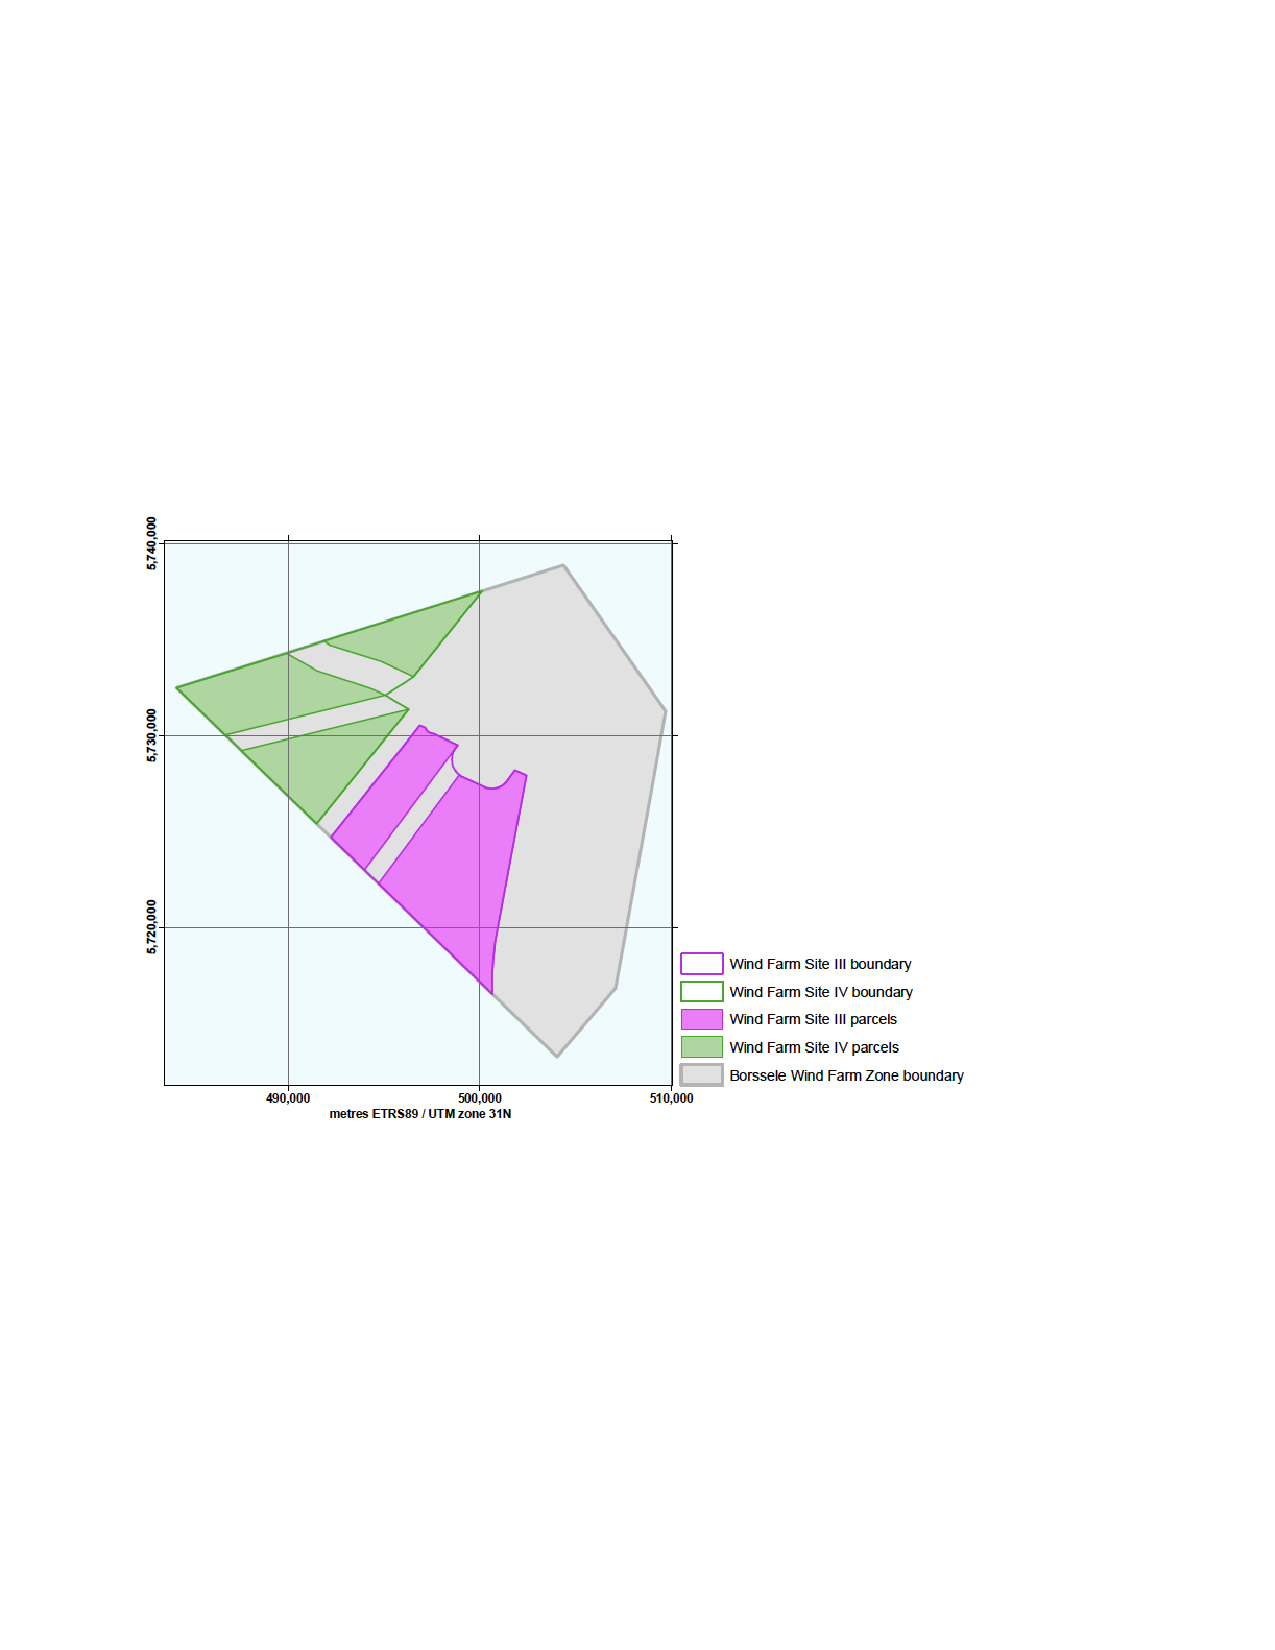
\includegraphics[width=0.9\textwidth, trim=0.9in 3.4in 2.0in 3.3in, clip]{./figures/BorselleBoundary.pdf} % second figure itself
		\caption{Borssele farm outline as presented in the NEA's document calling for bids.\cite{BorsseleAnnouncement}}
		\label{fig:farmoutline}
	\end{minipage}\hfill
	\begin{minipage}{0.45\textwidth}
		\centering
		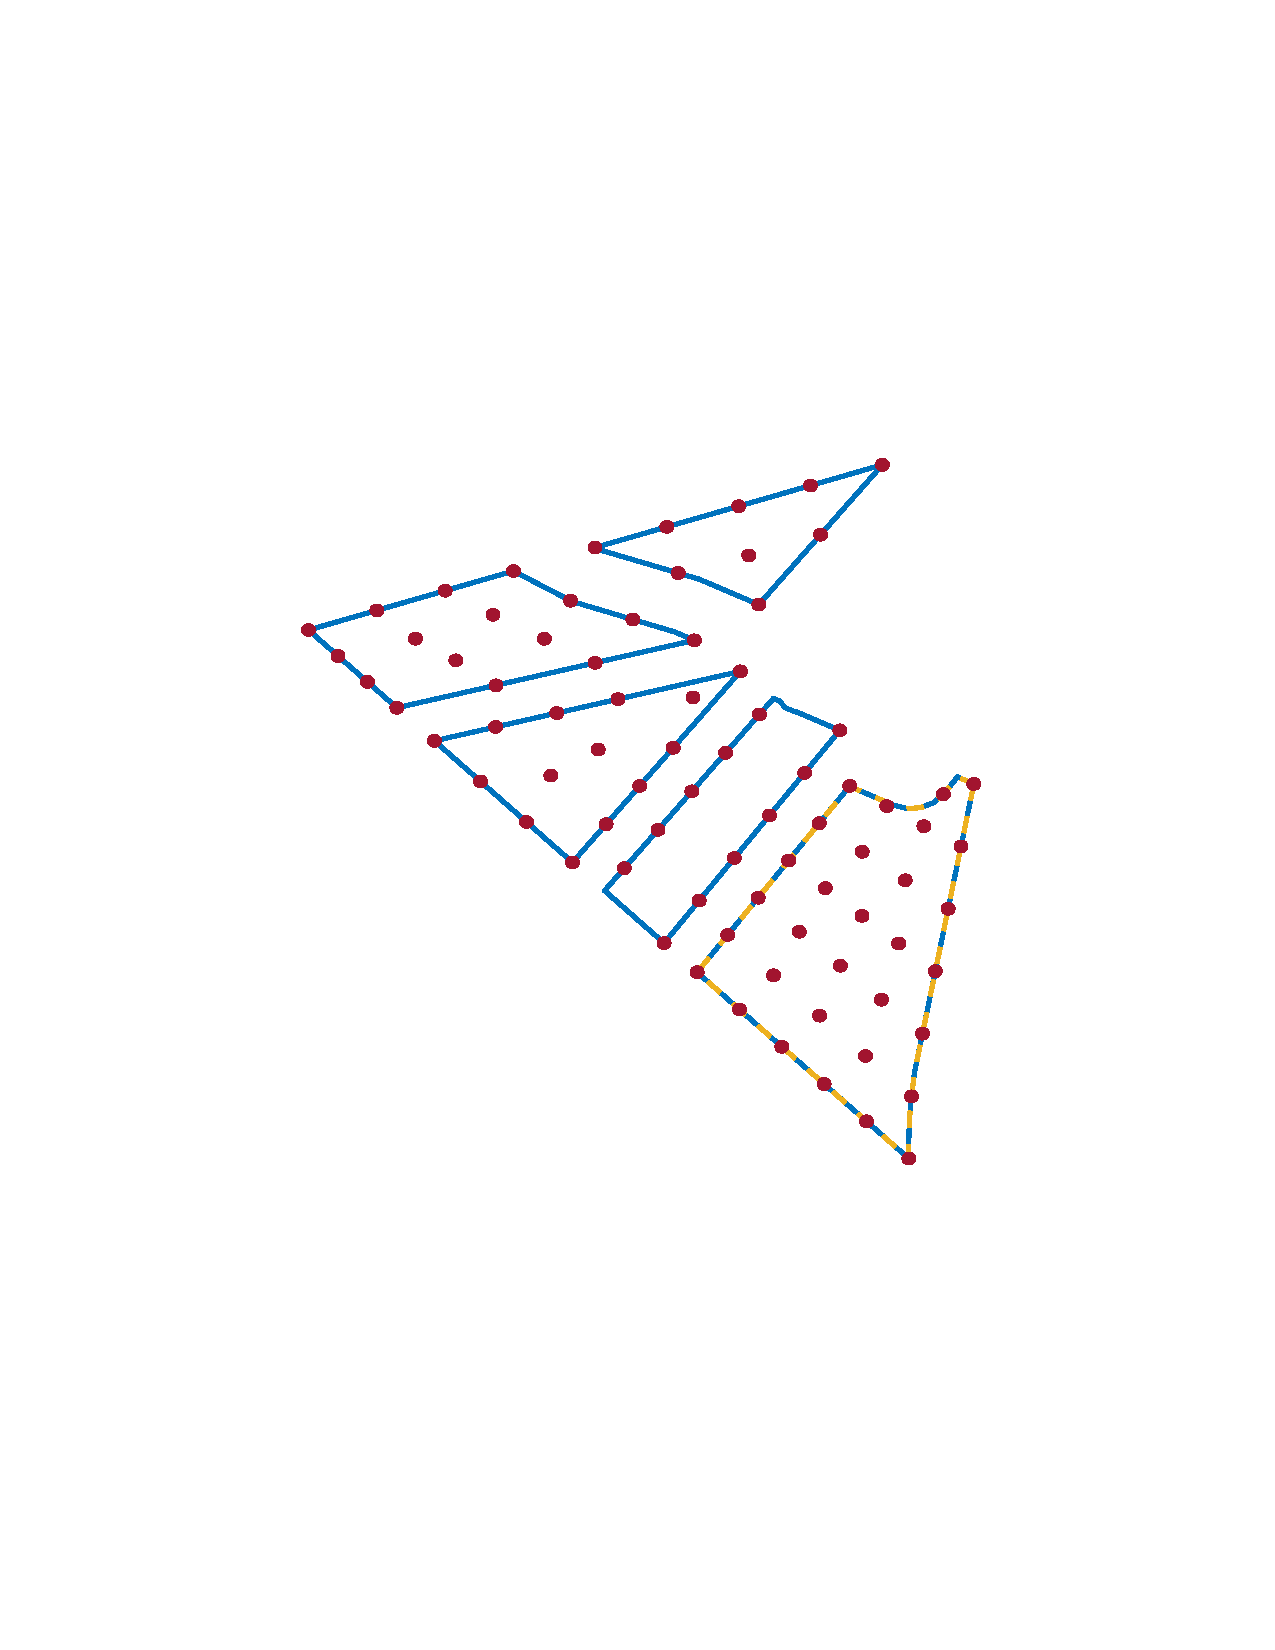
\includegraphics[width=0.9\textwidth, trim=0.8in 2.5in 1.0in 2.9in, clip]{./figures/cs4-layout.pdf} % first figure itself
		\caption{Graphical depiction of the boundaries and example layout we used for cs3 and cs4. The only boundary segment used in cs3 is in the bottom right, denoted by a dashed yellow and blue boundary.}
		\label{fig:ex4}
	\end{minipage}
\end{figure}

The first two case studies gave a simplified wind resource of sixteen (16) discrete bins and a constant wind speed across all directions.
To increase realism in cs3 \& cs4 we gave participants twenty (20) discrete directional bins, with twenty (20) wind speed probabilities at each bin, giving four-hundered (400) pieces of wind information in cs3 \& cs4 as opposed to the sixteen (16) given in cs1 \& cs2.

For cs3 the goal was to isolate variability in participants' optimization methods.
In order to do this we pre-coded a representative wake model as a control variable and permitted participants to use any optimization strategy they desire to alter turbine locations that would deliver the best annual energy production (AEP) for the farm.
We used only parcel IIIa of the Borssele farm in cs3, since it includes concavities but avoids the disjoint boundary problem.

The cs4 boundary invloved five parcels from the Borssele farm.
Besides adding the complexity of disjoint boundary sections, we also permitted participants to use whatever wake model they chose for optimization purposes, though final comparisons would be conducted with our supplied model.
The wake model we supplied was used in cs1, and is a modification of Bastankhah's Gaussian wake model.
The continuity of this wake model's output permits use of both gadient and non-gradient based optimization methods.
%Common and unique characteristics to each case study are presented below.

\bigskip
\subsection{Common to Both Case Studies} \label{sec:windfarm}

	\import{./sections/}{iea37-cs34-mthd-allcs.tex}
	
\subsection{Case Study 3: Non-Convex Boundary} \label{sec:cs3}

	\import{./sections/}{iea37-cs34-mthd-cs3.tex}

\subsection{Case Study 4: Discreet Boundary Regions with Concavities} \label{sec:cs4}

	\import{./sections/}{iea37-cs34-mthd-cs4.tex}